\documentclass[times]{article}

\usepackage[margin=1.0in]{geometry}
\usepackage{graphicx}
\usepackage{adjustbox}
\usepackage{float}
\usepackage{placeins}
\usepackage[none]{hyphenat}
\usepackage{amsmath}
\usepackage[us]{datetime}
\usepackage[explicit]{titlesec}
\usepackage{standalone}
\maxdeadcycles=100000
\begin{document}
	\title{”COMP SCI 5401 FS2017 Assignment 2a}
	\author{Dalton Cole \\ drcgy5@mst.edu}
	\date{\formatdate{5}{11}{2017}}
	\maketitle

	\section{Random Search}
	For this experiment, implementing a random genetic programming search of the Prisoner's Dilemma was required. Evaluations vs Fitness Plot can be seen in Figure \ref{fig:plot}. The tree visual can be seen in Figure \ref{fig:tree}.

	\begin{figure}
		\caption{Eval vs Fitness Plot}
		\label{fig:plot}
		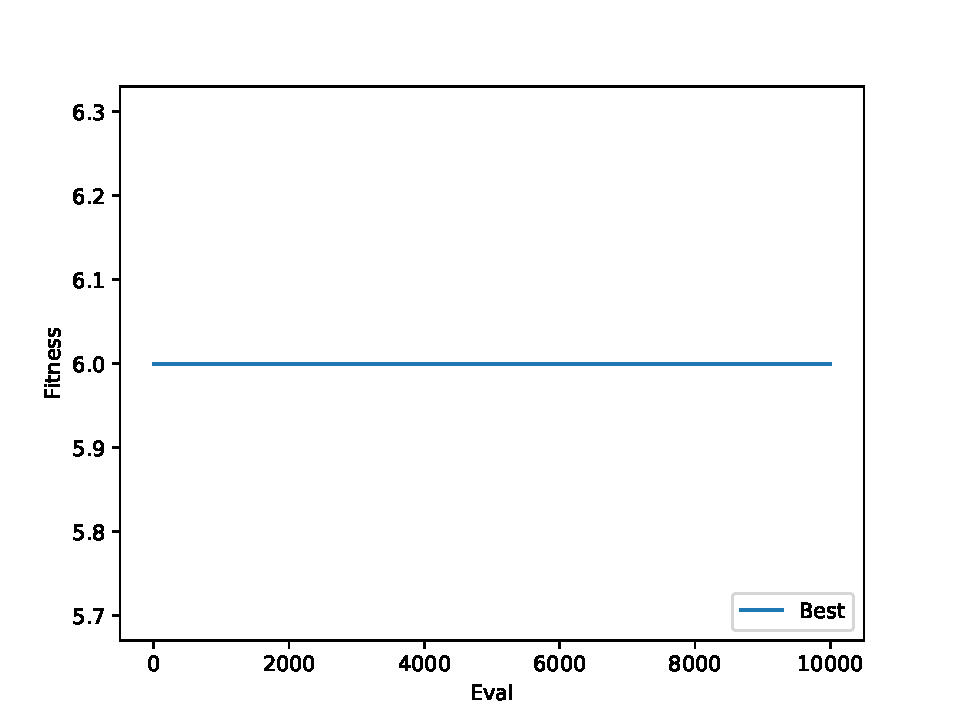
\includegraphics[width=\textwidth]{../graph/chart/0.pdf}
	\end{figure}

	\begin{figure}
		\caption{Tree Visualization}
		\label{fig:tree}
		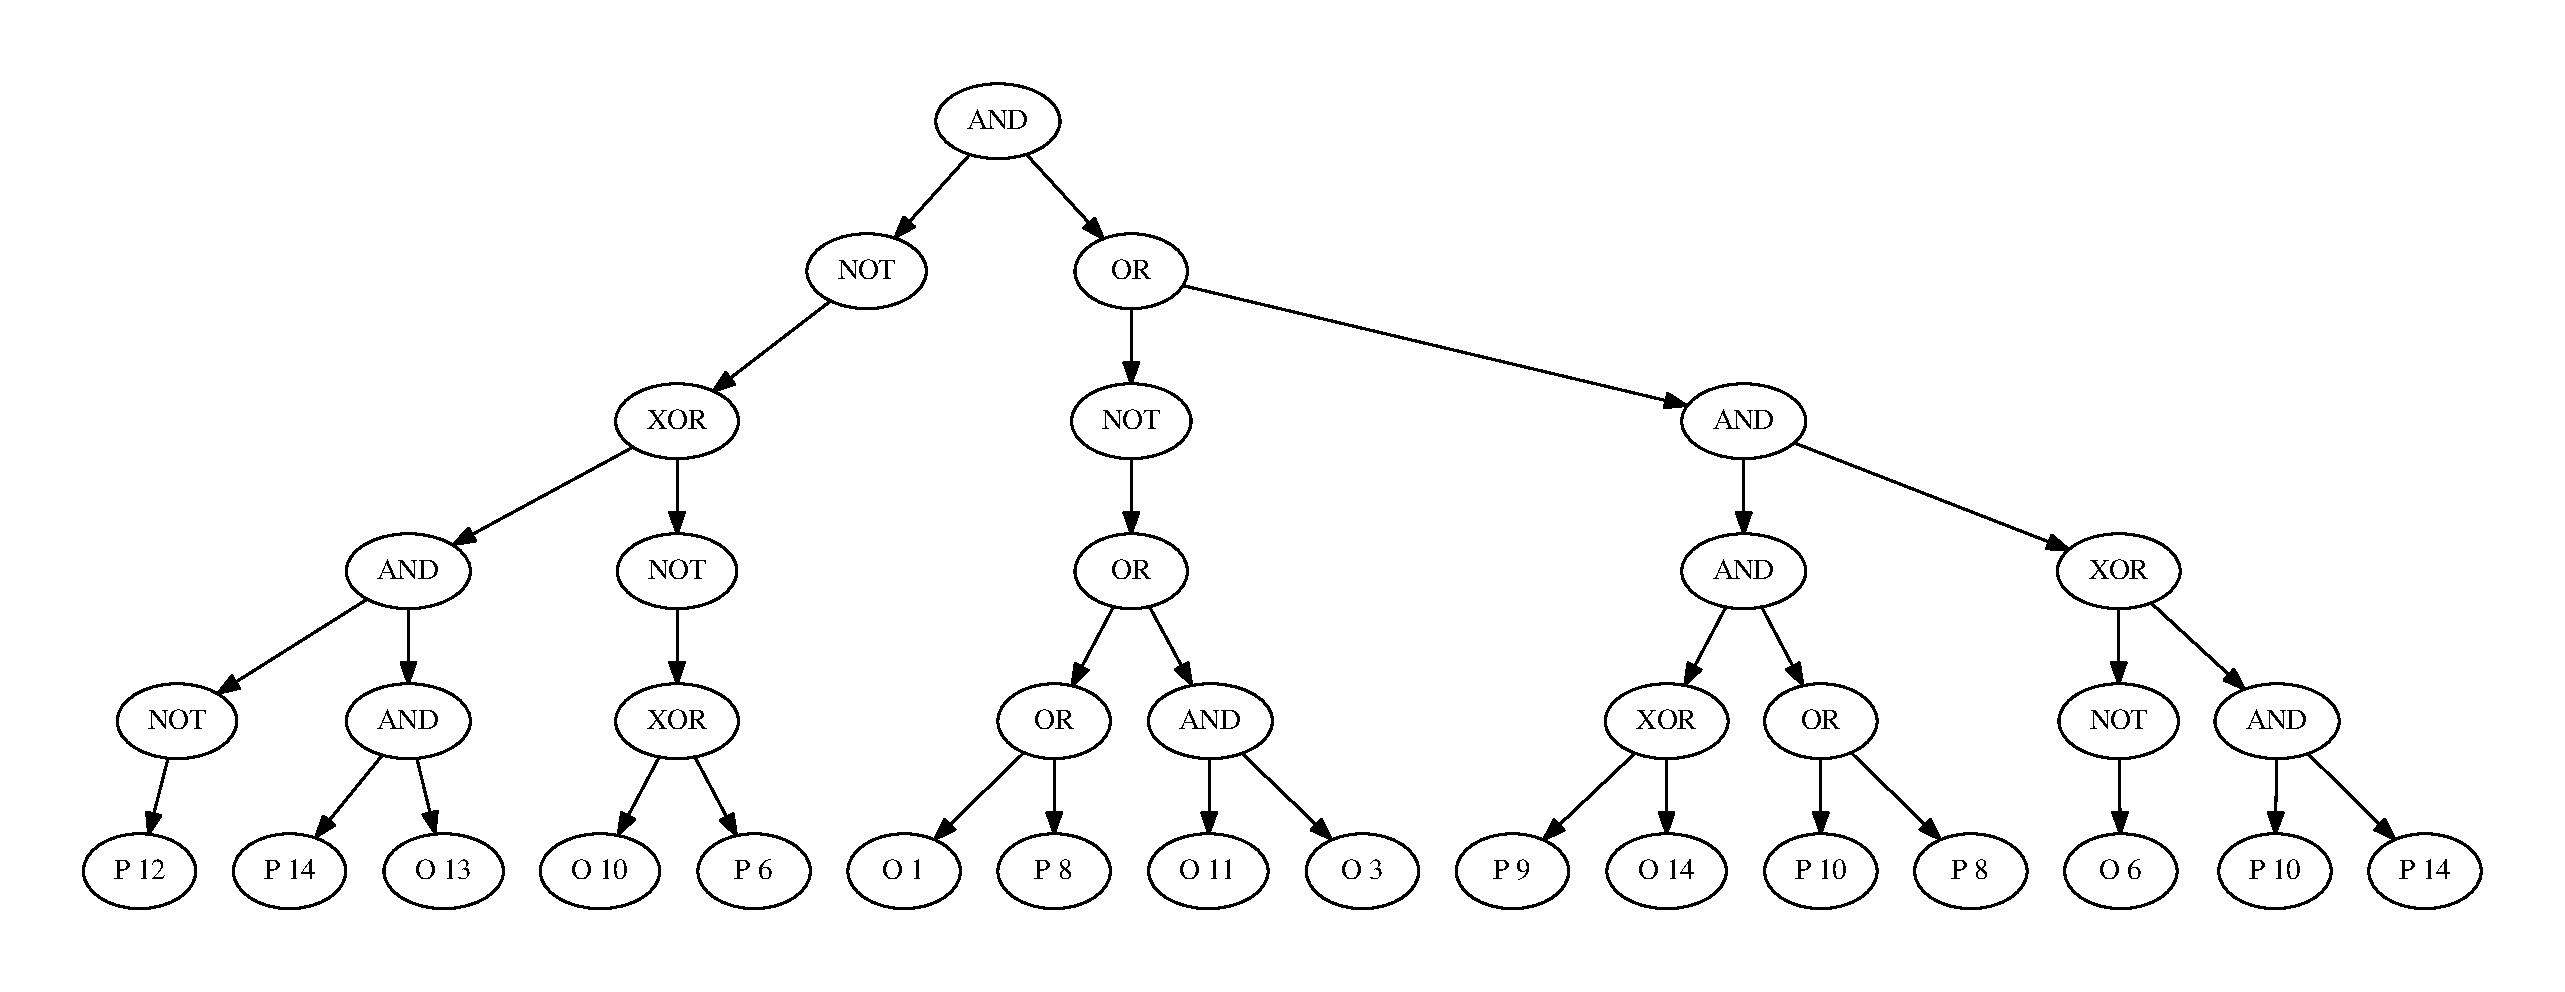
\includegraphics[angle=90,origin=c,width=\textwidth,height=\textheight]{../graph/tree/0.pdf}
	\end{figure}


		
\end{document}
